\section{Описание алгоритма} \label{section:algorithm}

Существует большое количество методов, позволяющих решать данную задачу. Методы, основанные на GAN (генеративно-состязательных) сетях \cite{gan-1},\cite{3d-gan} и VAE (вариацонном автоэнкодировщике) \cite{adversarial-autoencoder}, \cite{3d-autoencoder},\cite{lrgm-cloud}, не могут быть применены для решения данной задачи, по причине крайне малого (для задачи глубинного обучения) размера выборки. К примеру, в работе \cite{lrgm-cloud} при обучении на одну категорию используется более 1000 объектов. Более того, далеко не все архитектуры нейронных сетей позволяют на вход передавать облака точек с разными количествами вершин. В работе \cite{lrgm-cloud} авторы принудительно ограничивают вход сети определенным количеством точек. Стоит отметить, что в данном случае, можно было бы использовать специальные свертки , чтобы преодолеть подобные ограничения. 

В связи с вышеперечисленными фактами в данной работе мы будем использовать алгоритм, частично основанный на идеях
\textit{статистического анализа форм объектов (Statisitical shape spaces analysis)}.



Пусть у нас имеется выборка облаков точек размерности $M$.

\subsection{Выравнивание объектов (Alignment)}

Вначале все объекты в выборке необходимо выравнить. То есть, сделать так, чтобы ориентация всех зубов была одинаковой.
Задача оптимального совместного положения геометрических объектов широко известна и хорошо изучена. В общем случае задачу можно сформулировать следующим образом: пусть у нас имеется два облака точек $A$ и $B$. Необходимо найти матрицу поворота $R$, вектор сдвига $t$ и коэффициент размера $s$, такие что при применении их к объекту $B$ значение метрики расстояния между объектами стало минимальным. Обычно говорят токльо о нахождении матрицы поворота. В общем случае мы не обговариваем о какой именно метрике идет речь.

В данной задаче возможны два случая: случай, когда имеется имеется взаимно однозначное соответствие точек двух объектов, и случай, когда его нет.

\subsubsection{Случай наличия взаимно однозначного соответствия точек двух объектов}
Пусть у нас имеются два объекта, причем для каждой точки $a_{i}$ первого объекта $A = \{a_{1}, \ldots, a_{N}\}$, существует соответствующая точка $b_{i}$ второго объекта $B = \{b_{1}, \ldots, b_{N}\}$. Наличие данного соответствия отражается в функции расстояния между объектами (из соответствующей точке первого объекта вычисляется соответствующая точка второго объекта): $D(A, B) = \sum_{k=1}^{N}  \norm{a_{k} - b_{k}}_{2}^{2}$. 

Тогда задача поиска матрицы поворота в точности является \textit{задачей Вахба (Wahba's problem)} \cite{wahba}, которая заключается в нахождении матрицы поворота $R$, минимизирующей функция ошибки \[I(\textbf{R}) = \sum_{k=1}^{N}  \norm{a_{k} - \textbf{R} \, b_{k}}_{2}^{2} \]. Также существует \textit{ортогональная задача Прокрустеса (Orthogonal Procrustes problem)}, являющаяся аналогичной поставленной задаче.

\subsubsection{Случай отсутствия взаимно однозначного соответствия точек двух объектов}

В случае отсутствия взаимно однозначного соответствия задача выглядит следующим образом: пусть у нас имеются два объекта $A = \{a_{1}, \ldots, a_{N}\}$ и $B = \{b_{1}, \ldots, b_{K}\}$. Требуется найти такую матрицу $R$, чтобы функция ошибки \[I(\textbf{R}) = \sum\limits_{a \in A} \norm{a - \textbf{R} \, \textit{closest}(a, B)} \], где $\textit{closest}(a, B) = \argmin\limits_{b_{1}, \dots , b_{K}} \norm{a - b}$ принимала минимальное значение.


Данная задача в точности является задачей выравнивания множеств точек (point set registration, point). Данная задача хорошо изучена и существуют различные алгоритмы для ее решения.

Одним из таких алгоритмов является ICP алгоритм \cite{icp-main}, \cite{icp-2}. Он имеет две версии: rigid ICP и non-rigid ICP. Первая форма использует только жесткие преобразования (поворот, масштабирование и перенос), вторая же форма использует весь спектр аффинных преобразований. Идея алгоритма заключается в итеративной оценке и итеративном преобразовании (поворот, масштабирование и т.д.) исходных объектов.

Так-как функции ошибки зависит от взаимного положения объектов, то она модет меняться по ходу алгоритма. В связи с этим сложно доказать достижения локального оптимума алгоритмом. На самом деле, ICP в большинстве случаев не достигает локальных минимум функции ошибки \cite{icp-non-min}. Тем не менее, благодаря своей простоте, данный алгоритм остается самым распространенным алгоритмом для задачи выравнивания объектов.

Существуют также и другие алгоритмы: алгоритм надежного сопоставления точек (Robust point matching), алгоритм корреляции ядер (Kernel correlation).

% увеличение списка литература


\subsubsection{Выбор алгоритма}
Так-как в выборке нету однозначного соответствтия между точками (более того, объекты выборки имеют разные количества вершин), то мы будем использовать ICP алгоритм. Самой простой версии алгоритма - rigid ICP оказалось достаточно и в дальнейшем мы ее будем называть ICP.


\subsection{Нахождение общего порядка точек}

В дальнейших шагах алгоритма нам понадобится иметь общий порядок точек для всех облаков, то есть требуется найти взаимнооднозначное соответствие между вершинами облаков точек. Предыдущий шаг, во многом был нужен именно для того, чтобы процедура поиска соответствющий точек выполнялась как можно точнее. 


Для этого мы из выборки выбираем  облако точек с наименьшим количеством вершин (все равно больше соответствий мы найти не сможем). Если такие объектов будет несколько, то выбираем среди них один случайным образом. Будем называть найденное облако точек \textit{референсным}.


Теперь опишем процедуру поиска соответствия между вершинами для двух облаков точек. Пусть на вход передаются два облака точек, причем второе имеет меньше либо равное количество вершин чем первое облако. Для каждой вершины во втором облаке мы ищем ближайшую к нему вершину в первом облаке, и ставим их в однозначное соответствие. Разумеется, что часть точек первого облака мы потеряем, более того, возможно, что нескольким разным вершинам из второго облака будут соответствовать одинаковые вершины из первого.


Выполним описанную выше процедуру для каждого объекта из выборки и референсного облака. Теперь, у нас есть взаимно однозначные соответствия вершин для всех облаков в выборке. Вершинами, которым не были найдены соответствующие вершины референсного облака - отбрасываются.

В итоге, мы задаем некоторый случайный порядок вершин на референсном облаке, и, имея взаимно однозначное соответствие вершин для всех объектов из выборки, мы получаем порядок для вершин облаков из выборки.

Несмотря на то, что данный подход весьма прост, на имеющейся выборке он показывает хорошие результаты (в данном случае, большую роль играет выровненность объектов и их однородность).

% УВЕЛИЧЕНИЕ ОБЪЕМА!! придумать и вставить картинку

\subsection{Снижение размерности и анализ главных компонент}

Имея порядок вершин и их одинаковое количество для всех облака, мы превращаем облака точек в вектора, согласно порядку и получаем матрицы рамзерности $(N \times 3)$. Затем мы конкатенируем строчки данных матриц и получаем вектора размерности $(3N)$.

Сформируем матрицу из этих векторов. В итоге, у нас получится матрица $V \in \real^(M \times 3N)$.

Теперь, к этой матрице можно применить алгоритм \textit{PCA (Principal Component Analysis)} \cite{bishop} и получить в результате значения главных компонент.

Стоит отметить, что одной из форм постановки задачи PCA является задача поиска собственных значений и собственных векторов ковариационной матрицы (auto-covariance matrix): 
\[\Sigma = [\sigma_{ij}], \sigma_{ij} = \frac{1}{m - 1} \sum\limits_{l=1}^{m}(x_{li} - \bar{X_{i}})((x_{lj} - \bar{X_{j}}))\]

где собственные значения матрицы будут являться главными компонентами, а собственные вектора матрицы - главными значениями. 

Данная ковариационная матрица является обобщением понятия дисперсии для многомерной случайной величины. В связи с этим квадратные корни главных компонент или квадратные корни собственных значений матрицы являются стандартными отклонениями данных вдоль осей главных значений. Будем обозначать их через $\sigma$.

% X = (X_1, ... X_n) - multiple random value => s_ij = cov(X_i, X_j) = ... 
% Для вычисления  s_ij по имеющимся данным: для X_1 - m примеров то как в примере заменяем на выборочное среднее


Получив значения главных компонент, можно проанализировать насколько каждая компонента важна, для этого все главные компоненты упорядочиваются в порядке убывания: $\lambda_{1} \ge \lambda_{2} \ge \dots \ge \lambda_{M}$.
Необходимо выбрать первые $K$ компонент, которые будут сильно больше, чем последующие $M - K$ компонент. Примеры распределения главных компонент представлен на рис. \ref{fig:pcd-ex-1}, \ref{fig:pcd-ex-2}. Как можно будет увидеть дальше, для выборки зубов 
оптимальной областью значений $K$ является диапазон от 6 до 9 включительно.

\begin{figure*}[ht!]
    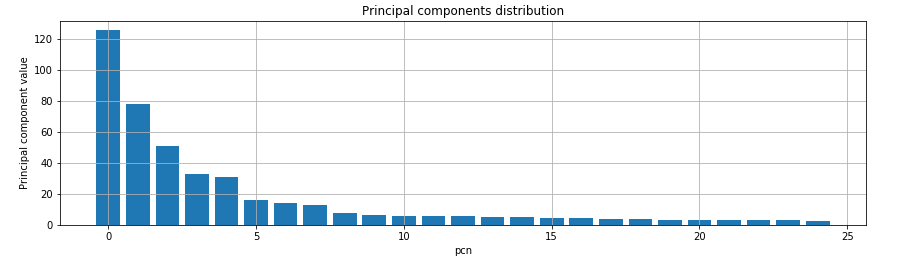
\includegraphics[width=1\linewidth]{images/pcd-example-1.png}
	\caption{Пример распределения значений главных компонент}
    \label{fig:pcd-ex-1}
\end{figure*}

\begin{figure*}[ht!]
    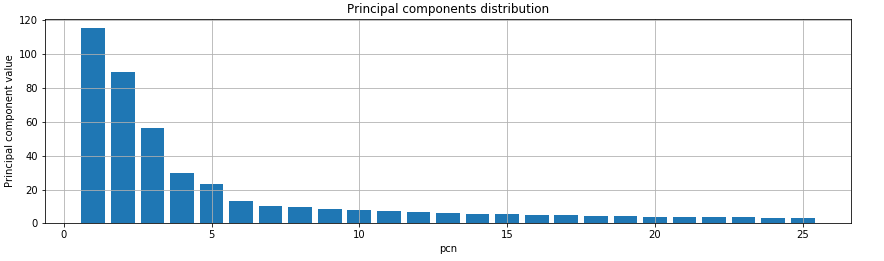
\includegraphics[width=1\linewidth]{images/pcd-example-2.png}
	\caption{Пример распределения значений главных компонент}
    \label{fig:pcd-ex-2}
\end{figure*}


\subsection{Генерация новых объектов}

На предыдущем шаге мы оставили $K$ главных компонент. Каждой главная i-ой компоненте соответствует стандартное отклонение $\sigma_{i}$. То есть, из них можно сформировать вектор стандартных отклонений $\overline{\sigma} = \{\sigma_{1}, \dots, \sigma_{K}\}$. 


В итоге можно семплировать случайные вектора с диапазоном $\pm c \cdot \overline{\sigma}$, где c - некоторая константа. В дальнейшем будет показано, что значения $c \ge 3$ не дают особого прироста к точности (что хорошо коррелирует с правилом трех сигм).


